\chapter{Function Compositions}

Given $f(x) = x - 5$, $g(x) = 4 + \sqrt{2x+1}$, and $h(x) = \dfrac{3}{x+7}$, simplify each \underline{and state the domain}.
\begin{enumerate}
	\item $(f \circ g)(x)$
	\item $(g \circ f)(x)$
	\item $h(h(x))$
\setcounter{Review}{\value{enumi}}
\end{enumerate}

Find each of the following given the table below.
\begin{center}
\begin{tabular}{c|c|c|c|c|c|c|c|c|c}
    $\bm{x}$ & $\bm{-4}$ & $\bm{-3}$ & $\bm{-2}$ & $\bm{-1}$ & \textbf{0} & \textbf{1} & \textbf{2} & \textbf{3} & \textbf{4} \\ \hline
    $\bm{f(x)}$ & $-3$ & 0 & $-1$ & 3 & 1 & 2 & 4 & $-4$ & $-2$ \\ \hline
    $\bm{g(x)}$ & 3 & $-1$ & 0 & 1 & 4 & $-2$ & $-4$ & 2 & $-3$ \\
\end{tabular}
\end{center}

\begin{multicols}{5}
\begin{enumerate}	\setcounter{enumi}{\value{Review}}
\item $(f \circ g)(-1)$
\item $(g \circ g)(0)$
\item $(f \circ f)(2)$
\item $(g \circ g)(-3)$
\item $f(g(0))$
\setcounter{Review}{\value{enumi}}
\end{enumerate}
\end{multicols}

Use the table below to answer each.
\begin{center}
    \begin{tabular}{|c|c|c|c|c|c|c|c|c|c|c|}
    \hline 
        $x$ & $-4$ & $-3$ & $-2$ & $-1$ & 0 & 1 & 2 & 3 & 4 \\ \hline 
        $f(x)$ & 1 & $-1$ & $-2$ & 4 & 0 & $-4$ & $-3$ & 3 & 2 \\ \hline 
        $g(x)$ & 0 & $-2$ & 1 & $-4$ & $-3$ & 2 & $-1$ & 4 & 3 \\ \hline 
    \end{tabular}
\end{center}

\begin{multicols}{5}
\begin{enumerate}	\setcounter{enumi}{\value{Review}}
\item $(f \circ g)(-1)$
\item $f(g(3))$
\item $(g \circ f)(0)$
\item $f(f(4))$
\item $g(f(g(1)))$
\setcounter{Review}{\value{enumi}}
\end{enumerate}
\end{multicols}

Given $f(x) = \sqrt{3x+2}$, $g(x) = x^2 - 1$, and $h(x) = 9x-2$, find each of the following.
\begin{enumerate}
\setcounter{enumi}{\value{Review}}
\item $(g \circ f)(x)$
\item $f(g(x))$
\item $(h \circ h)(x)$
\setcounter{Review}{\value{enumi}}
\end{enumerate}

Find each of the following given the graphs of $f(x)$ (in red) and $g(x)$ (in blue) below:    \newline\\

\begin{center}
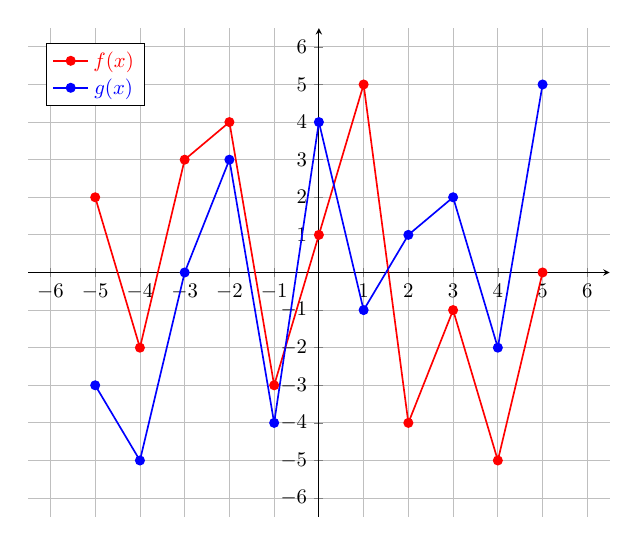
\begin{tikzpicture}[scale=0.75]
\begin{axis}
[xmin=-6.5, xmax=6.5, ymin=-6.5, ymax=6.5, xtick distance = 1, ytick distance = 1, axis lines=center, grid, width=4.5in, legend pos={north west}]
\addplot[color=red, mark=*, thick] coordinates {
(-5, 2) (-4,-2) (-3,3) (-2,4) (-1,-3) (0,1) (1,5) (2,-4) (3,-1) (4,-5) (5,0)
};
\addplot[color=blue, mark=*, thick] coordinates {
(-5, -3) (-4,-5) (-3,0) (-2,3) (-1,-4) (0,4) (1,-1) (2,1) (3,2) (4,-2) (5,5)
};
\addlegendentry{{\color{red}$f(x)$}};
\addlegendentry{{\color{blue}$g(x)$}};
\end{axis}
\end{tikzpicture}
\end{center}

\begin{multicols}{5}
\begin{enumerate}   \setcounter{enumi}{\value{Review}}  
    \item $(f \circ g)(-1)$
    \item $(g \circ f)(-4)$
    \item $f(g(3))$
    \item $g(g(-2))$
    \item $(f \circ f)(-5)$
\end{enumerate} \setcounter{Review}{\value{enumi}}
\end{multicols}

Given $f(x) = \sqrt{2x-9}$ and $g(x) = \frac{2x}{x-3}$, simplify each and state the domain of the composition.

\begin{multicols}{3}
\begin{enumerate}	\setcounter{enumi}{\value{Review}}  
    \item $f(g(x))$
    \item $(g \circ f)(x)$
    \item $g(g(x))$
\end{enumerate}		\setcounter{Review}{\value{enumi}}
\end{multicols}

\newpage

\section{Answer Key}

\begin{enumerate}
	\item $-1 + \sqrt{2x+1}$ Domain: $\left[-\frac{1}{2}, \infty\right)$
	\item $4 + \sqrt{2x-9}$ Domain: $\left[\frac{9}{2}, \infty\right)$
	\item $\frac{3x+21}{7x+52}$ Domain: $\left(-\infty, -\frac{52}{7}\right) \cup \left(-\frac{52}{7}, -7\right) \cup (-7, \infty)$
	\item 2
     \item $-3$
     \item $-2$
     \item 1
     \item $-2$
     \item 1
     \item 2
     \item $-3$
     \item $-3$
     \item $-2$
     \item $3x + 1$
    \item $\sqrt{3x^2-1}$
    \item $81x-20$
    \item $-2$
    \item 3
    \item $-4$
    \item 2
    \item $-4$
    \item $f(g(x)) = \sqrt{\frac{-5x+27}{x-3}}; \quad \left(3, \frac{27}{5}\right]$
    \item $(g \circ f)(x) = \frac{2\sqrt{2x-9}}{\sqrt{2x-9}-3}; \quad \left[\frac{9}{2},9\right) \cup (9, \infty)$
    \item $g(g(x)) = \frac{4x}{9-x}; \quad (-\infty, 3) \cup (3, 9) \cup (9, \infty)$
\end{enumerate}